\documentclass{CInf_practice}

\sheet{5}{Programmierbare Bausteine, Hazards und Flipflops}
\begin{document}
\cinftitle

\ex{Bit-Slice-ALU}{6 + 8 + 16 + 4 = 34}
\subex{}
\begin{tabular}{cc|ccc||cc}
   $s_1$ & $s_0$ & $a_i$ & $b_i$ & $c_{i-1}$ & $y_i$ & $c_i$ \\\hline
0 & 0 & 0 & 0 & 0 & 0 & 0 \\
0 & 0 & 0 & 0 & 1 & 1 & 0 \\
0 & 0 & 0 & 1 & 0 & 1 & 0 \\
0 & 0 & 0 & 1 & 1 & 0 & 1 \\
0 & 0 & 1 & 0 & 0 & 1 & 0 \\
0 & 0 & 1 & 0 & 1 & 0 & 1 \\
0 & 0 & 1 & 1 & 0 & 0 & 1 \\
0 & 0 & 1 & 1 & 1 & 1 & 1 \\
0 & 1 & 0 & 0 & 0 & 0 & 0 \\
0 & 1 & 0 & 0 & 1 & 1 & 1 \\
0 & 1 & 0 & 1 & 0 & 1 & 1 \\
0 & 1 & 0 & 1 & 1 & 0 & 1 \\
0 & 1 & 1 & 0 & 0 & 1 & 0 \\
0 & 1 & 1 & 0 & 1 & 0 & 0 \\
0 & 1 & 1 & 1 & 0 & 0 & 0 \\
0 & 1 & 1 & 1 & 1 & 1 & 1 \\
1 & 0 & 0 & 0 & 0 & 0 & X \\
1 & 0 & 0 & 0 & 1 & 0 & X \\
1 & 0 & 0 & 1 & 0 & 0 & X \\
1 & 0 & 0 & 1 & 1 & 0 & X \\
1 & 0 & 1 & 0 & 0 & 0 & X \\
1 & 0 & 1 & 0 & 1 & 0 & X \\
1 & 0 & 1 & 1 & 0 & 1 & X \\
1 & 0 & 1 & 1 & 1 & 1 & X \\
1 & 1 & 0 & 0 & 0 & 1 & X \\
1 & 1 & 0 & 0 & 1 & 1 & X \\
1 & 1 & 0 & 1 & 0 & 1 & X \\
1 & 1 & 0 & 1 & 1 & 1 & X \\
1 & 1 & 1 & 0 & 0 & 0 & X \\
1 & 1 & 1 & 0 & 1 & 0 & X \\
1 & 1 & 1 & 1 & 0 & 0 & X \\
1 & 1 & 1 & 1 & 1 & 0 & X 
\end{tabular}

\subex{}
$y_i$:
\begin{center}
\begin{tikzpicture}
   \matrix (m)[
      nodes={matrix node},
      matrix of nodes,
      inner sep=0pt,
      outer sep=0pt,
      row sep=-.5pt,
      column sep=-.5pt
   ]  {
      0 & 1 & 0 & 1 & 0 & 0 & 0 & 0 \\
      1 & 0 & 1 & 0 & 1 & 1 & 0 & 0 \\
      1 & 0 & 1 & 0 & 0 & 0 & 1 & 1 \\
      0 & 1 & 0 & 1 & 0 & 0 & 1 & 1 \\
   };
  
   \clip ($(m.north west) + (-8pt,8pt)$) rectangle ($(m.south east) + (8pt,-8pt)$);
   \draw[|-|] ($(m-1-5.north west) + (0,2.2cm)$) -- node[above] () {$s_1$} ($(m-1-8.north east) + (0,2.2cm)$);
   \draw[|-|] ($(m-1-3.north west) + (0,1.4cm)$) -- node[above] () {$a_i$} ($(m-1-6.north east) + (0,+1.4cm)$);
   \draw[|-|] ($(m-1-2.north west) + (0,.6cm)$) -- node[above] () {$c_{i-1}$} ($(m-1-3.north east) + (0,0.6cm)$);
   \draw[|-|] ($(m-1-6.north west) + (0,.6cm)$) -- node[above] () {$c_{i-1}$} ($(m-1-7.north east) + (0,0.6cm)$);
   \draw[|-|] ($(m-2-1.north west) + (-.6cm,0)$) -- node[left] () {$b_i$} ($(m-3-1.south west) + (-.6cm,0)$);
   \draw[|-|] ($(m-3-1.north west) + (-1.2cm,0)$) -- node[left] () {$s_0$} ($(m-4-1.south west) + (-1.2cm,0)$);

   \draw[highlight,draw=red] ($(m-2-1.north west) + (3pt,-3pt)$) rectangle ($(m-3-1.south east) + (-3pt,3pt)$);
   \draw[highlight] ($(m-2-3.north west) + (3pt,-3pt)$) rectangle ($(m-3-3.south east) + (-3pt,3pt)$);
   \draw[highlight,draw=olive,dashed] ($(m-4-2.north west) + (3pt,-3pt)$) rectangle ($(m-4-2.south east) + (-3pt,-1cm)$);
   \draw[highlight,draw=olive,dashed] ($(m-1-2.south east) + (-3pt,3pt)$) rectangle ($(m-1-2.north west) + (3pt,1cm)$);
   \draw[highlight,loosely dashed] ($(m-4-4.north west) + (3pt,-3pt)$) rectangle ($(m-4-4.south east) + (-3pt,-1cm)$);
   \draw[highlight,loosely dashed] ($(m-1-4.south east) + (-3pt,3pt)$) rectangle ($(m-1-4.north west) + (3pt,1cm)$);
   \draw[highlight] ($(m-2-5.north west) + (3pt,-3pt)$) rectangle ($(m-2-6.south east) + (-3pt,3pt)$);
   \draw[highlight] ($(m-3-7.north west) + (3pt,-3pt)$) rectangle ($(m-4-8.south east) + (-3pt,3pt)$);
\end{tikzpicture}
$y_i = \comp s_1\comp a_i \comp b_i c_{i-1} + \comp s_1 \comp a_i b_i \comp
c_{i-1} + \comp s_1 a_i \comp b_i \comp c_{i-1} + \comp s_1 a_i b_i c_{i-1} + s_1
\comp s_0 a_i b_i + s_1 s_0 \comp a_i$
\end{center}

$c_i$:
\begin{center}
\begin{tikzpicture}
   \matrix (m)[
      nodes={matrix node},
      matrix of nodes,
      inner sep=0pt,
      outer sep=0pt,
      row sep=-.5pt,
      column sep=-.5pt
   ]  {
      0 & 0 & 1 & 0 & X & X & X & X \\
      0 & 1 & 1 & 1 & X & X & X & X \\
      1 & 1 & 1 & 0 & X & X & X & X \\
      0 & 1 & 0 & 0 & X & X & X & X \\
   };
  
   \clip ($(m.north west) + (-8pt,8pt)$) rectangle ($(m.south east) + (8pt,-8pt)$);
   \draw[|-|] ($(m-1-5.north west) + (0,2.2cm)$) -- node[above] () {$s_1$} ($(m-1-8.north east) + (0,2.2cm)$);
   \draw[|-|] ($(m-1-3.north west) + (0,1.4cm)$) -- node[above] () {$a_i$} ($(m-1-6.north east) + (0,+1.4cm)$);
   \draw[|-|] ($(m-1-2.north west) + (0,.6cm)$) -- node[above] () {$c_{i-1}$} ($(m-1-3.north east) + (0,0.6cm)$);
   \draw[|-|] ($(m-1-6.north west) + (0,.6cm)$) -- node[above] () {$c_{i-1}$} ($(m-1-7.north east) + (0,0.6cm)$);
   \draw[|-|] ($(m-2-1.north west) + (-.6cm,0)$) -- node[left] () {$b_i$} ($(m-3-1.south west) + (-.6cm,0)$);
   \draw[|-|] ($(m-3-1.north west) + (-1.2cm,0)$) -- node[left] () {$s_0$} ($(m-4-1.south west) + (-1.2cm,0)$);

   \draw[highlight,draw=red] ($(m-3-2.north east) + (-3pt,-3pt)$) rectangle ($(m-3-1.south east) + (-3cm,3pt)$);
   \draw[highlight,draw=red] ($(m-3-7.north west) + (3pt,-3pt)$) rectangle ($(m-3-8.south east) + (3cm,3pt)$);
   \draw[highlight,dashed] ($(m-3-2.north west) + (3pt,-3pt)$) rectangle ($(m-4-2.south east) + (-3pt,3pt)$);
   \draw[highlight,dashed] ($(m-3-7.north west) + (3pt,-3pt)$) rectangle ($(m-4-7.south east) + (-3pt,3pt)$);
   \draw[highlight,draw=blue,dash dot] ($(m-2-2.north west) + (3pt,-3pt)$) rectangle ($(m-3-3.south east) + (-3pt,3pt)$);
   \draw[highlight,draw=blue,dash dot] ($(m-2-6.north west) + (3pt,-3pt)$) rectangle ($(m-3-7.south east) + (-3pt,3pt)$);
   \draw[highlight,draw=olive] ($(m-1-3.north west) + (3pt,-3pt)$) rectangle ($(m-2-3.south east) + (-3pt,3pt)$);
   \draw[highlight,draw=olive] ($(m-1-6.north west) + (3pt,-3pt)$) rectangle ($(m-2-6.south east) + (-3pt,3pt)$);
   \draw[highlight,draw=teal,dashed] ($(m-2-3.north west) + (3pt,-3pt)$) rectangle ($(m-2-6.south east) + (-3pt,3pt)$);
\end{tikzpicture}

$c_i = b_i c_{i-1} + \comp s_0 a_i b_i + s_0 \comp a_i c_{i-1} + s_o \comp a_i
b_i + \comp s_0 a_i c_{i-1}$
\end{center}

\subex{}

\newlength{\vlinedist}
\newlength{\hlinedist}
\newlength{\hcablelength}
\newlength{\vcablelength}
\newlength{\radius}

\setlength{\vlinedist}{.4cm}
\setlength{\hlinedist}{.3cm}
\setlength{\hcablelength}{32\vlinedist}
\setlength{\vcablelength}{11\hlinedist}
\setlength{\radius}{1.5pt}

\usetikzlibrary{intersections,calc,positioning}
\tikzstyle{inverter}=[font=\tiny,minimum height=.3cm,
   text width=.3cm,rectangle,anchor=center,
   align=center,
   inner sep=0,
draw ]
\tikzstyle{and gate}=[rectangle,font=\small,align=center,draw,fill=white,inner
sep=1pt,minimum height=.7em]
\begin{center}
   \begin{tikzpicture}
      \foreach \x in {1,...,10}
      {
         \draw[name path global/.expanded=h \x] (0,\hlinedist*\x) --
         ++(\hcablelength,0);
      }
      \foreach \x in {0,...,31} {
         \draw[name path global/.expanded=v \x] (\vlinedist*\x, \vcablelength)
         node[name=v \x start] {} -- ++(0,-\vcablelength-5*\hlinedist);
         \node[and gate] at ($(v \x start) + (0,-\vcablelength-\hlinedist)$) {\&};
      }
      \foreach \x / \y in {1/s_1,2/s_0,3/c_{i-1},4/a_i,5/b_i}
      {
         \node[anchor=east] (\y) at ($(0,\vcablelength+\hlinedist-2\hlinedist*\x) + (-1cm,0)$) {$\y$};
         \node[inverter,below right=\hlinedist-.15cm-.5\pgflinewidth and .8\vlinedist of \y.east] (inv-\y) {1};
         \draw (\y) -- ++(5cm,0);
         \node[draw,shape=circle,inner sep=.5pt,right=0pt-\pgflinewidth of inv-\y] (inv-\y-circle) {};
         \draw (inv-\y-circle) -- ++(1cm,0);
         \draw (inv-\y.west) -| ($(\y.east) + (.3\vlinedist,0)$);
         \fill[black] ($(\y.east) + (.3\vlinedist,0)$) circle (\radius);
      }
      \draw[name path=yi] (-\vlinedist,-2.5\hlinedist) -- ++(\hcablelength+\vlinedist,0) node[and gate] {$\ge$} -- +(1em,0) ++(2em,0) node {$y_i$};
      \draw[name path=ci] (-\vlinedist,-4\hlinedist) -- ++(\hcablelength+\vlinedist,0) node[and gate] {$\ge$} -- +(1em,0) ++(2em,0) node {$c_i$};
      \node[rectangle,draw,very thick,below=2\hlinedist of b_i] {\textbf{PROM}};

      %% DRAW THE DOTS
      \newcounter{num}
      \foreach \line[count=\x,evaluate=\line as \l using int(\line-1),
         evaluate=\line as \t using int(\line+1),
      ] in {1,3,5,...,10}{
         %% ODD ROWS %%%%%%%%%%%%%%%%
         \pgfmathsetmacro{\numdots}{pow(2,\x-1)}
         \ifthenelse{\line=1}{
            \foreach \c in {0,2,...,30}{
               \fill[name intersections={of={h \line} and {v \c}}] (intersection-1) circle (\radius);
            }
         }{
            \setcounter{num}{0}
            \whiledo{\value{num}<32}{
               \foreach \n in {1,...,\numdots}{
                  \ifthenelse{\value{num}<32}{\fill[name intersections={of={h \line} and {v \arabic{num}}}] (intersection-1) circle (\radius);
                     \stepcounter{num}
                  }{}
               }
               \foreach \n in {1,...,\numdots}{\stepcounter{num}}
            }
         }
         %% END ODD ROWS %%%%%%%%%%%%

         %% EVEN ROWS %%%%%%%%%%%%%%%%
         \ifthenelse{\line=1}{
            \foreach \c in {0,2,...,30}{
               \pgfmathsetmacro{\index}{int(pow(2,\x-1)+\c)}
               \fill[name intersections={of={h \t} and {v \index}}] (intersection-1) circle (\radius);
            }
         }{
            \setcounter{num}{0}
            \whiledo{\value{num}<32}{
               \foreach \n in {1,...,\numdots}{
                  \pgfmathsetmacro{\index}{int(pow(2,\x-1)+\value{num})}
                  \ifthenelse{\index<32 \AND \value{num}<32}{\fill[name
                     intersections={of={h \t} and {v \index}}] (intersection-1) circle (\radius);
                     \stepcounter{num}
                  }{}
               }
               \foreach \n in {1,...,\numdots}{\stepcounter{num}}
            }
         }
         %% END EVEN ROWS %%%%%%%%%%%%
      }
      %% DOTS IN OR MATRIX
      \foreach \x in {1,2,4,7,9,10,12,15,19,23,26,27,30,31}{
      \fill[name intersections={of=yi and {v \x}}] (intersection-1) circle (\radius);
      }
      %% DOTS IN OR MATRIX
      \foreach \x in {3,5,6,7,9,12,13,15,19,21,22,23,25,28,29,31}{
      \fill[name intersections={of=ci and {v \x}}] (intersection-1) circle (\radius);
      }
   \end{tikzpicture}
\end{center}

\addtolength{\hcablelength}{-20\vlinedist}
\begin{center}
   \begin{tikzpicture}
      \foreach \x in {1,...,10}
      {
         \draw[name path global/.expanded=h \x] (0,\hlinedist*\x) --
         ++(\hcablelength,0);
      }
      \foreach \x in {0,...,11} {
         \draw[name path global/.expanded=v \x] (\vlinedist*\x, \vcablelength)
         node[name=v \x start] {} -- ++(0,-\vcablelength-5*\hlinedist);
         \node[and gate] at ($(v \x start) + (0,-\vcablelength-\hlinedist)$) {\&};
      }
      \foreach \x / \y in {1/s_1,2/s_0,3/c_{i-1},4/a_i,5/b_i}
      {
         \node[anchor=east] (\y) at ($(0,\vcablelength+\hlinedist-2\hlinedist*\x) + (-1cm,0)$) {$\y$};
         \node[inverter,below right=\hlinedist-.15cm-.5\pgflinewidth and .8\vlinedist of \y.east] (inv-\y) {1};
         \draw (\y) -- ++(5cm,0);
         \node[draw,shape=circle,inner sep=.5pt,right=0pt-\pgflinewidth of inv-\y] (inv-\y-circle) {};
         \draw (inv-\y-circle) -- ++(1cm,0);
         \draw (inv-\y.west) -| ($(\y.east) + (.3\vlinedist,0)$);
         \fill[black] ($(\y.east) + (.3\vlinedist,0)$) circle (\radius);
      }
      \draw[name path=yi] (-\vlinedist,-2.5\hlinedist) -- ++(\hcablelength+\vlinedist,0) node[and gate] {$\ge$} -- +(1em,0) ++(2em,0) node {$y_i$};
      \draw[name path=ci](-\vlinedist,-4\hlinedist) -- ++(\hcablelength+\vlinedist,0) node[and gate] {$\ge$} -- +(1em,0) ++(2em,0) node {$c_i$};
      \node[rectangle,draw,very thick,below=2\hlinedist of b_i] {\textbf{PAL}};

      %% DRAW THE DOTS
      \foreach \x / \y in
      {1/0,1/2,2/1,2/3,2/4,2/6,2/7,2/9,3/0,3/1,3/5,3/8,3/9,4/2,4/3,4/4,4/7,4/10,5/1,5/2,6/0,6/3,6/6,6/8,6/10,7/4,7/7,7/10,8/5,8/8,8/9,9/0,9/1,9/2,9/3,10/4,10/5}{
         \fill[name intersections={of={h \x} and {v \y}}] (intersection-1) circle (\radius);
      }
      \foreach \x[evaluate=\x as \y using int(\x+6)] in {0,...,5} {
         \fill[name intersections={of=yi and {v \x}}] (intersection-1) circle (\radius);
         \fill[name intersections={of=ci and {v \y}}] (intersection-1) circle (\radius);
      }
   \end{tikzpicture}
   \begin{tikzpicture}
      \foreach \x in {1,...,10}
      {
         \draw[name path global/.expanded=h \x] (0,\hlinedist*\x) --
         ++(\hcablelength,0);
      }
      \foreach \x in {0,...,11} {
         \draw[name path global/.expanded=v \x] (\vlinedist*\x, \vcablelength)
         node[name=v \x start] {} -- ++(0,-\vcablelength-5*\hlinedist);
         \node[and gate] at ($(v \x start) + (0,-\vcablelength-\hlinedist)$) {\&};
      }
      \foreach \x / \y in {1/s_1,2/s_0,3/c_{i-1},4/a_i,5/b_i}
      {
         \node[anchor=east] (\y) at ($(0,\vcablelength+\hlinedist-2\hlinedist*\x) + (-1cm,0)$) {$\y$};
         \node[inverter,below right=\hlinedist-.15cm-.5\pgflinewidth and .8\vlinedist of \y.east] (inv-\y) {1};
         \draw (\y) -- ++(5cm,0);
         \node[draw,shape=circle,inner sep=.5pt,right=0pt-\pgflinewidth of inv-\y] (inv-\y-circle) {};
         \draw (inv-\y-circle) -- ++(1cm,0);
         \draw (inv-\y.west) -| ($(\y.east) + (.3\vlinedist,0)$);
         \fill[black] ($(\y.east) + (.3\vlinedist,0)$) circle (\radius);
      }
      \draw[name path=yi] (-\vlinedist,-2.5\hlinedist) -- ++(\hcablelength+\vlinedist,0) node[and gate] {$\ge$} -- +(1em,0) ++(2em,0) node {$y_i$};
      \draw[name path=ci](-\vlinedist,-4\hlinedist) -- ++(\hcablelength+\vlinedist,0) node[and gate] {$\ge$} -- +(1em,0) ++(2em,0) node {$c_i$};
      \node[rectangle,draw,very thick,below=2\hlinedist of b_i] {\textbf{PLA}};

      %% DRAW THE DOTS
      \foreach \x / \y in
      {1/0,1/2,2/1,2/3,2/4,2/6,2/7,2/9,3/0,3/1,3/5,3/8,3/9,4/2,4/3,4/4,4/7,4/10,5/1,5/2,6/0,6/3,6/6,6/8,6/10,7/4,7/7,7/10,8/5,8/8,8/9,9/0,9/1,9/2,9/3,10/4,10/5}{
         \fill[name intersections={of={h \x} and {v \y}}] (intersection-1) circle (\radius);
      }
      \foreach \x[evaluate=\x as \y using int(\x+6)] in {0,...,5} {
         \fill[name intersections={of=yi and {v \x}}] (intersection-1) circle (\radius);
         \ifthenelse{\y=11}{}{\fill[name intersections={of=ci and {v \y}}] (intersection-1) circle (\radius);
         }
      }
   \end{tikzpicture}
\end{center}
\subex{}

Offensichtlich sind AND- sowie OR-Matrix beim PROM deutlich größer, da sie alle
$2^5$ Minterme abdeckt und daher keinen Profit aus dem Verschmelzen von
Mintermen schlägt. Beim PAL und PLA hingegen ist die Größe der AND-Matrix
so angepasst, dass fast genau die benötigte Anzahl Terme realisiert werden kann. Das
PAL spart gegenüber dem PROM 20 Verknüpfungen in der OR-Matrix. Das PLA-Netz
kann eine weitere Verknüpfung einsparen, da ein Draht tatsächlich redundant ist
und damit auch nicht in der OR-Matrix verbunden werden muss.




\ex{Taktsteuerung von D-Flipflops}{8+8+8=24}
\begin{center}
\noindent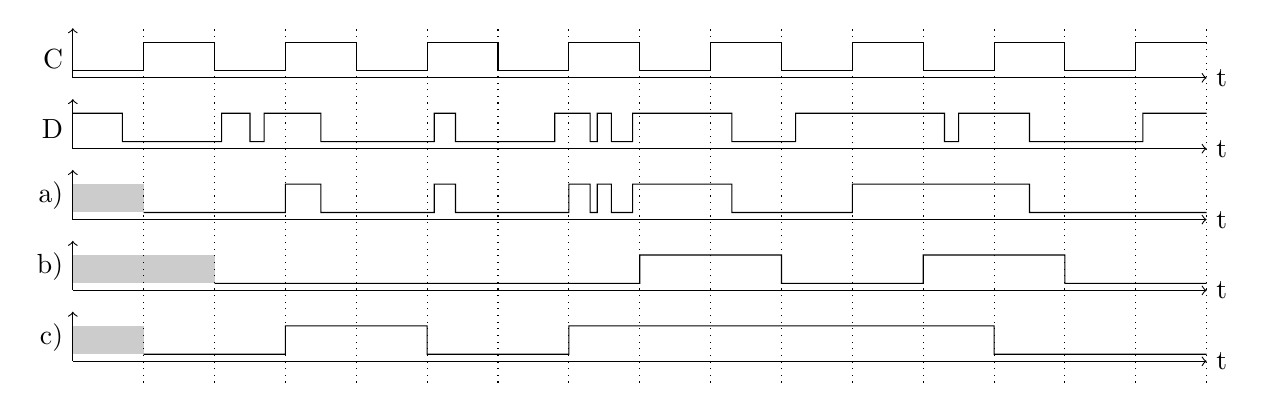
\begin{tikzpicture}[scale=.9]

% helpers
\def\hAzero{2.4}  \def\hAone{2.8}
\def\hBzero{1.4}  \def\hBone{1.8}
\def\hCzero{0.4}  \def\hCone{0.8}
\def\hCyzero{4.4} \def\hCyone{4.8}
\def\hDzero{3.4}  \def\hDone{3.8}

\def\diff{.4}

% undefs
\def\drawundef#1#2{\fill[gray!40] (0, #1) rectangle ++(#2, -\diff);}
\drawundef{\hAone}{1}
\drawundef{\hBone}{2}
\drawundef{\hCone}{1}

% grid
\foreach \name/\y in {C/5,D/4,a)/3,b)/2,c)/1}{
  \draw[<-] (0,\y) -- ++(0,-.7) node[anchor=south east] {\name};
}
\foreach \y in {.3,1.3,2.3,3.3,4.3}{
  \draw[->] (0,\y) -- ++(16,0) node[anchor=west] {t};
}
\foreach \x in {1,...,16}{
  \draw[dotted] (\x, 0) -- ++(0,5);
}

% draw helpers
\def\drawAt#1#2{\draw (#1,#2) -- ++(1,0);}
\def\connect#1#2{\draw (#2,#1) -- ++(0,\diff);}

% draw cycle
\foreach \x in {0,2,...,15}{
  \drawAt{\x}{\hCyzero}
  \connect{\hCyzero}{\x}
}
\foreach \x in {1,3,...,15}{
  \drawAt{\x}{\hCyone}
  \connect{\hCyzero}{\x}
}

% draw D
\def\up{, \hDzero) -- ++(0, \diff) -- (}
\def\dn{, \hDone)  -- ++(0, -\diff) -- (}
\draw (0, \hDone) -- (.7 \dn 2.1 \up 2.5 \dn 2.7 \up 3.5 \dn 5.1 \up 5.4 \dn 
                     6.8 \up 7.3 \dn 7.4 \up 7.6 \dn 7.9 \up 9.3 \dn 10.2 \up
                     12.3 \dn 12.5 \up 13.5 \dn 15.1 \up 16, \hDone);

% draw A
\def\up{, \hAzero) |- ++(0, \diff) -- (}
\def\dn{, \hAone)  -- ++(0, -\diff) -- (}
\draw (1, \hAzero) -- (3 \up 3.5 \dn 5.1 \up 5.4 \dn 7 \up 7.3 \dn 7.4 \up 7.6 \dn 7.9 \up 9.3 \dn 11 \up
 13.5 \dn 16, \hAzero);

% draw B
\def\up{, \hBzero) -- ++(0, \diff) -- (}
\def\dn{, \hBone)  -- ++(0, -\diff) -- (}
\draw (2, \hBzero) -- (8 \up 10 \dn 12 \up 14 \dn 16, \hBzero);

% draw C
\def\up{, \hCzero) -- ++(0, \diff) -- (}
\def\dn{, \hCone)  -- ++(0, -\diff) -- (}
\draw (1, \hCzero) -- (3 \up 5 \dn 7 \up 13 \dn 16, \hCzero);


\end{tikzpicture}
\end{center}























\end{document}
